\documentclass[11pt]{report}
\usepackage{amsmath}
\usepackage{amssymb}
\usepackage{amsfonts}
\usepackage{mathtools}
\usepackage{amsthm}
\usepackage{ragged2e}
\usepackage[hidelinks]{hyperref}
\usepackage{float}
\usepackage{pgf,tikz}
\usepackage[shortlabels]{enumitem}
\usepackage{color}
\usepackage{pgfplots}
\usepackage[margin = 1 in]{geometry}
\usepackage{mathrsfs}
\usetikzlibrary{arrows}
\usepackage{multicol}
\usepackage{fancyhdr}
\pagestyle{fancy}
\usepackage{multirow}
\usepackage{graphicx}
\usepackage{psfrag}
\usepackage{listings}
\renewcommand{\footrulewidth}{0.4pt}

\newtheorem{theorem}{Theorem}[chapter]
\newtheorem{defn}{Definition}[chapter]
\newtheorem{lemma}{Lemma}[chapter]

\theoremstyle{definition}
\newtheorem{proposition}{Proposition}[chapter]
\newtheorem{remark}{Remark}[chapter]
\newtheorem{example}{Example}[chapter]

\newcommand{\user}{}
\newcommand{\xlr}[2]{#1 \left(#2\right)}
\newcommand{\clr}[2]{#1 \left\{ #2 \right\}}
\newcommand{\rank}{\mathrm{rank}}
\newcommand{\mat}[1]{\mathbf{#1}}
\lhead{ECE 530 - Fall 2023 at University of Illinois at Urbana-Champaign}
\rhead{HW3}
\lfoot{Author: \textcolor{red}{Eric Silk, esilk2}}
\rfoot{Due: Wednesday, Sep 27}
\begin{document}


\section*{Problem 1: Can you fit a line?}
\subsection*{Problem Statement}
Consider $N$ data points $(\mathbf{x}_i, y_i)$ for $i=1,\ldots,N$ obtained from
an experiment , where $\mathbf{x}_i\in\mathbb{R}^n$ and $y_i\in\mathbb{R}$. Let
$N>n+1$. The goal of linear regression is to find the ``best'' linear fit; i.e.
find $\mathbf{c}\in\mathbb{R}^n$, $d\in\mathbb{R}$ s.t.:
\[y_i\approx \mathbf{c}^T\mathbf{x}_i + d,\ \textrm{for}\ i=1,\ldots,N\]

\subsubsection*{a}
Suppose each measurement is corrupted by independent Gaussian noise with
identical variances and 0 mean. Find $\mathbf{A}\in\mathbb{R}^{N\times(n+1)}$ in
terms of $\mathbf{x}_1,\ldots,\mathbf{x}_N$ s.t. that the maximum likelihood
estimate of $\hat{\mathbf{c}}$, $\hat{d}$ is
\[
	\begin{pmatrix}
		\hat{\mathbf{c}} \\
		\hat{d}
	\end{pmatrix}
	=
	\left(\mathbf{A}^T\mathbf{A}\right)^{-1}\mathbf{A}^Ty,\
	\textrm{where}\ \mathbf{y}\coloneqq
	\begin{pmatrix}
		y_1    \\
		\vdots \\
		y_N
	\end{pmatrix}
\]

\subsubsection*{b}
Consider the case with $n=1$; i.e. $x_1,\ldots,x_N$ are scalars. Finding the best linear fit amounts to finding
$(\hat{c}, \hat{d})$ tht minimizes:
\[ J(c,d) \coloneqq \sum_{i=1}^{N}(y_i-cx_i-d)^2 \]
Compute a stationary point $(\hat{c},\hat{d})$ by setting the derivative of $J$ w.r.t $c$ and $d$ to zero.

\subsubsection*{c}
Use the second derivative tests to conclude that your $(\hat{c}, \hat{d})$ computed in (b) is indeed a
local minimizer of $J$. Can you conclude from this second derivative test alone that it is a global minimizer?

\subsubsection*{d}
Consider the following $(x,y)$ pairs:
\begin{itemize}[itemsep=0pt]
	\item $(1.00, 1.10)$
	\item $(1.50, 1.62)$
	\item $(2.00, 1.98)$
	\item $(2.57, 2.37)$
	\item $(3.00, 3.23)$
	\item $(3.50, 3.69)$
	\item $(4.00, 3.97)$
\end{itemize}
Draw a scatter plot of these points; then, plot the best linear fit to these points using your formula in part (b).

\subsection*{Solution}
\subsubsection*{a}
We can rewrite the given equation to:
\[y_i = \mathbf{x}_i^T \mathbf{c} + d\]
Additionally, let: $\mathbf{1}_N$ be a column vector of 1's with $N$ rows.
Thus:
\[
	\mathbf{y} = \begin{pmatrix}
		\mathbf{x}_1 \\
		\vdots       \\
		\mathbf{x}_N
	\end{pmatrix}
	\mathbf{c} + d\mathbf{1}_N
\]
We can further re-arrange this to:
\[
	\mathbf{y} = \begin{pmatrix}
		\mathbf{x}_1 & 1      \\
		\mathbf{x}_2 & 1      \\
		\vdots       & \vdots \\
		\mathbf{x}_N & 1
	\end{pmatrix}
	\begin{pmatrix}
		\mathbf{c} \\
		d
	\end{pmatrix}
	\implies
	\mathbf{A} = \begin{pmatrix}
		\mathbf{x}_1 & 1      \\
		\mathbf{x}_2 & 1      \\
		\vdots       & \vdots \\
		\mathbf{x}_N & 1
	\end{pmatrix}
\]

\subsubsection*{b}
\[
	\nabla J(c, d) = \begin{pmatrix}
		\frac{\partial J}{\partial c} \\
		\frac{\partial J}{\partial d}
	\end{pmatrix}
	=
	2\begin{pmatrix}
		\sum_{i=1}^{N}\left(y_i-cx_i-d\right)(-x_i) \\
		\sum_{i=1}^{N}\left(y_i-cx_i-d\right)(-1)
	\end{pmatrix}
\]
Setting equal to zero and noting that the $2$ can then just drop out (and push the negative sign around):
\[
	\mathbf{0} = \begin{pmatrix}
		\sum_{i=1}^{N}\left(cx_i+d-y_i\right)(x_i) \\
		\sum_{i=1}^{N}\left(cx_i+d-y_i\right)
	\end{pmatrix}
\]
Exanding the top:
\[
	0
	= \sum_{i=1}^N(cx_i^2+dx_i-y_ix_i)
	= c\left(\sum x_i^2\right) + d \left(\sum x_i\right) - \left(\sum x_iy_i\right)
\]
And the bottom:
\[
	0
	= \sum_{i=1}^N(cx_i+d-y_i)
	= c\left(\sum x_i\right) + d\left(\sum 1\right) - \left(\sum y_i\right)
\]
Solve for $c$:
\[
	c = \left(\left(\sum y_i\right)- d\left(\sum 1\right)\right)/ \left(\sum x_i\right)
\]
Note that $\sum_{i=1}^N 1 = N$.
Plug into the first partial derivative equation:
\[ 0=\frac{\sum y_i - Nd}{\sum x_i} \sum x_i^2 + d\sum{x_i}-\sum{x_iy_i} \]
Solve for $d$:
\[ \frac{\sum x_i^2\sum y_i - Nd\sum x_i^2}{\sum x_i} + d\sum x_i - \sum x_iy_i \]
\[=\sum x_i^2\sum y_i - Nd\sum x_i^2 + d\left(\sum x_i\right)^2-\sum x_i\sum x_iy_i\]
\[Nd\sum x_i^2 - d\left(\sum x_i\right)^2 = \sum x_i^2\sum y_i - \sum x_i\sum x_iy_i\]
\[d \left(N\sum x_i^2 - \left(\sum x_i\right)^2\right) = \sum x_i^2\sum y_i - \sum x_i\sum x_iy_i\]
\[ d = \frac{\sum x_i^2\sum y_i - \sum x_i\sum x_iy_i}{N\sum x_i^2 - \left(\sum x_i\right)^2 } \]
which can then be plugged back in to get $c$. I'm lazy so I used Wolfram to
simplify the expression and got:
\[ c = \frac{\sum x_i\sum y_i - N \sum x_iy_i}{\left(\sum x_i\right)^2-N\sum x_i^2} \]

\subsubsection*{c}
Given the gradient, the Hessian is trivially calculable as:
\[
	\nabla^2 J(c,d) = 2\begin{pmatrix}
		\sum x_i^2 & \sum x_i \\
		\sum x_i   & N
	\end{pmatrix}
\]
If $\nabla^2 J \succcurlyeq 0$ everywhere then $J$ is convex and the first order
condition ($\nabla J = 0$) is sufficient for both a global and local optimality.
HOWEVER, this will ultimately depend on the $x$'s chosen, as well as the
quantity $N$ chosen. The eigenvalues are given by\footnote{Thanks, Wolfram!}:
\[
	\lambda_{1,2}
	= \frac{1}{2}
	\left(
	\sum x_i^2 + N \pm \sqrt{(\sum x_i^2)^2+4\sum (x_i)^2 +N^2-2N\sum x_i^2}
	\right)
\]
which must be $\lambda_{1,2} \geq 0$ for the matrix to be PSD. We know that
$N\geq1$ and $x_i\in\mathbb{R}\implies \sum x_i^2 \geq 0$, so for both
eigenvalues to be non-negative the following must hold:
\[\sum x_i^2 + N \geq \sqrt{\sum x_i^2 - 2N\sum x_i^2+4\left(\sum x_i\right)^2 + N^2}\]
Failing this condition, the matrix is not PSD and we cannot assume global
optimality (although it doesn't imply it is NOT a global optimum).

\newpage
\subsubsection*{d}
Code is made available at the end of document.
\begin{figure}[!h]
	\centering
	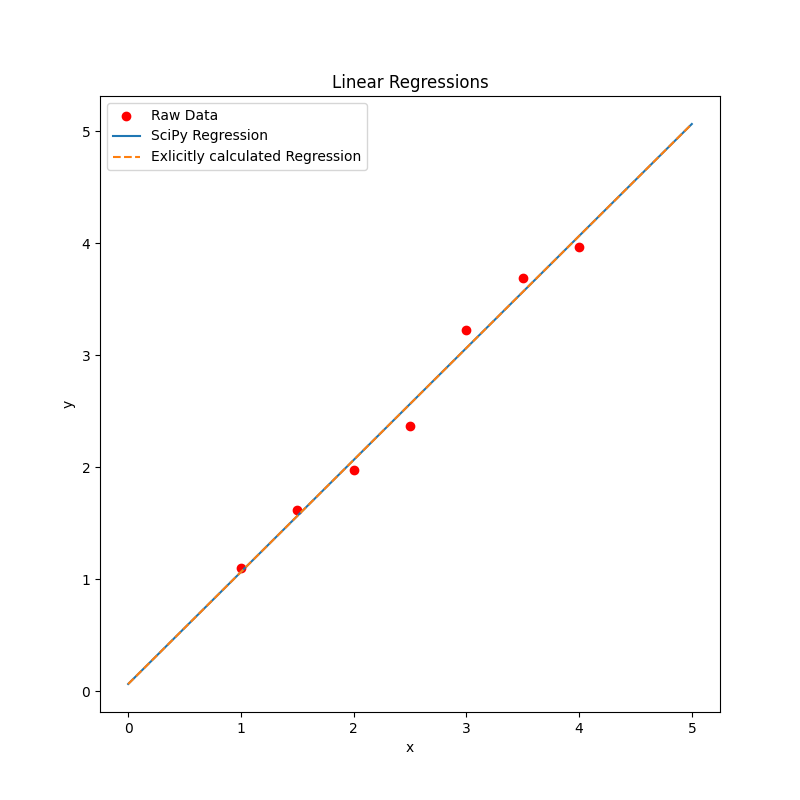
\includegraphics[width=\textwidth]{plots/hw3_regression.png}
	\caption{Linear Regression on the provided data, using both the derived
		expression (dashed orange line) and SciPy's built-in method for verification
		(solid blue line)}
\end{figure}


\section*{Problem 2: Estimate with Confidence}
\subsection*{Problem Statement}
Suppose the true parameters of a system are described by $x=(1,1)^T$, and the measurements
are given by:
\[
	\mat{y} = \underbrace{\begin{pmatrix}
			1 & 2 \\
			2 & 3 \\
			3 & 4 \\
			4 & 5
		\end{pmatrix}}_{\coloneqq A}
	\mat{x} + \mat{e}
\]
where $e\in\mathbb{R}^4$ is sampled from a multivariate Gaussian distribution with zero mean and covariance
matrix $\mat{R}\coloneqq \textrm{diag}(0.1, 0.2, 0.3, 0.4)$. That is, $\mat{e}\sim\mathcal{N}(0, \mat{R})$.
\subsubsection*{a}
Write code for the following experiment:
\begin{enumerate}
	\item Generate an error vector $\mat{e}$ according to $\mathcal{N}(0,\mat{R})$.
	      Compute $\mat{y}$ from it and report it.
	\item In class we derived a formula to compute the maximum likelihood
	      estimate $\hat{\mat{x}}$ from $\mat{y}$. Using $\mat{y}$ from the previous
	      step, compute and report your estimate $\hat{\mat{x}}$.
	\item The estimated error is given by $\mat{y}-\mat{A}\hat{\mat{x}}$. With
	      $\mat{y}$ from the prior steps, compute and report:
	      \[J(\hat{\mat{x}}) \coloneqq (\mat{y}-\mat{A}\hat{\mat{x}})^T\mat{R}^{-1}(\mat{y}-\mat{A}\hat{\mat{x}})\]
	      Recall that we claimed (without proof) that
	      $J(\hat{\mat{x}})\sim \chi_2^2$. Then, we have:
	      \[\mathbb{P}\left\{J(\hat{\mat{x}})\leq 5.9915\right\}=0.95\]
	      where $\mathbb{P}\left\{\mathcal{E}\right\}$ denotes the probability
	      of an event $\mathcal{E}$. Concludewith a $95\%$ confidence level
	      whether your estimate error conforms to the error model we assumed.
\end{enumerate}
\subsubsection*{b}
Repeat the experiment in the prior section TEN-THOUSAND TIMES. Each time you run
the experiment, record the value of $J(\hat{\mat{x}})$.  Plot a histogram of
$J(\hat{\mat{x}})$. Comment qualitatively how the histogram of
$J(\hat{\mat{x}})$ compares to the PDF of a $\chi_2^2$ random variable. Also,
report the percentage of times you concluded that your measurement did not
conform t the error model. Compare this fraction to your confidence interval in
the prior portion.

\subsection*{Solution}
\subsubsection*{a}
Again, code is made available at the end of the assignment. The output of the script is:
\lstinputlisting[basicstyle=\small]{plots/script_output.txt}

\subsubsection*{b}
\begin{figure}[!h]
	\centering
	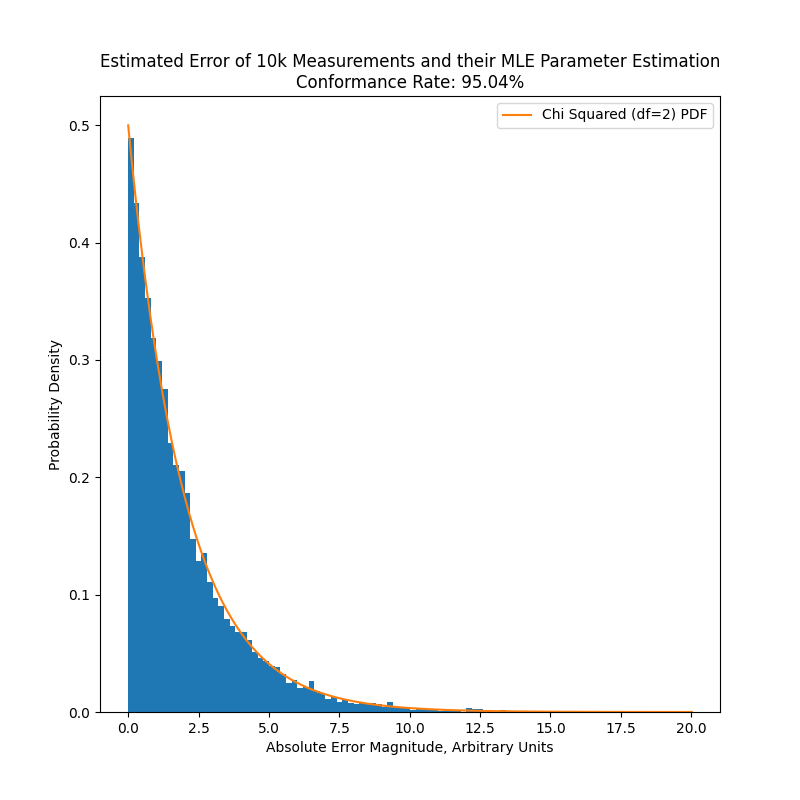
\includegraphics[width=\textwidth]{plots/problem2_hist.png}
	\caption{Density based histogram of 10k experiments with a 2-DoF Chi-Squared
		PDF superimposed. Qualitatively...pretty dang good!}
\end{figure}


\newpage
\section*{Code}
\definecolor{codegreen}{rgb}{0,0.6,0}
\definecolor{codegray}{rgb}{0.5,0.5,0.5}
\definecolor{codepurple}{rgb}{0.58,0,0.82}
\definecolor{backcolour}{rgb}{0.95,0.95,0.92}
\lstdefinestyle{mystyle}{
	backgroundcolor=\color{backcolour},
	commentstyle=\color{codegreen},
	keywordstyle=\color{magenta},
	numberstyle=\tiny\color{codegray},
	stringstyle=\color{codepurple},
	basicstyle=\ttfamily\footnotesize,
	breakatwhitespace=false,
	breaklines=true,
	captionpos=b,
	keepspaces=true,
	numbers=left,
	numbersep=5pt,
	showspaces=false,
	showstringspaces=false,
	showtabs=false,
	tabsize=2
}
\lstset{style=mystyle}
\lstinputlisting[
	language=Python,
	basicstyle=\tiny
]{../../ece530/ece530/hw3/__main__.py}

%------------------------------------------------------------------------------------------------------------

%------------------------------------------------------------------------------------------------------------

\end{document}
